% !TeX root = ../main.tex

\chapter{實驗設計與結果分析}

本章詳述實驗環境、資料集統計量、評估指標、對照組模型設定，以及完整的實驗結果分析，包含主要效能對比、消融實驗與可解釋性評估。

\section{實驗環境與資料集}

\subsection*{硬體與軟體環境}

所有實驗均在同一台配備 Intel Arc GPU (XPU) 的工作站上執行。模型以 PyTorch 框架實作，採用 BFloat16 混合精度訓練以加速運算並降低記憶體需求。深層模型（$L \geq 2$）另搭配梯度檢查點 (Gradient Checkpointing) 技術，確保訓練過程不因記憶體不足而中斷。

\subsection*{資料集}

本研究使用 Food.com 食譜推薦資料集~\cite{majumder2019foodcom}，該資料集包含使用者對食譜的評分紀錄、食譜的詳細屬性（包含食材、標籤、營養成分等）。經預處理後，我們將其轉化為隱式回饋形式。資料集統計量如表~\ref{tab:dataset} 所示。

\begin{table}[htbp]
  \centering
  \caption{Food.com 資料集統計量}
  \label{tab:dataset}
  \begin{tabular}{lr}
    \toprule
    項目 & 數量 \\
    \midrule
    使用者數 & 226,570 \\
    食譜數 & 231,637 \\
    互動紀錄數 & 1,132,367 \\
    互動稀疏度 & 99.9978\% \\
    \midrule
    KG 實體數（含食譜） & 15,370 \\
    KG 關係類型數 & 2 (食材、標籤) \\
    KG 三元組數 & 2,230,927 \\
    CKG 總節點數 & 473,577 \\
    CKG 總邊數（含反向） & 7,200,165 \\
    \bottomrule
  \end{tabular}
  \par\vspace{4pt}
  \begin{minipage}{0.9\linewidth}
    \footnotesize \textit{表中 KG 實體數與三元組數均為超級節點修剪後的數據：食材超級節點，即出現頻率前 0.5\%（74 個）及 13 個語義過於通用的基礎食材，已於前處理階段移除，詳見 §\ref{sec:supernode_pruning}；標籤超級節點（出現頻率前 50）亦同步移除。}
  \end{minipage}
\end{table}

\subsection*{超參數設定}

為確保實驗的公平性，所有模型皆採用統一的超參數設定，如表~\ref{tab:hyperparams} 所示。

\begin{table}[htbp]
  \centering
  \caption{實驗超參數設定}
  \label{tab:hyperparams}
  \begin{tabular}{ll}
    \toprule
    超參數 & 設定值 \\
    \midrule
    嵌入維度 (Embedding Dim) & 64 \\
    批次大小 (Batch Size) & 1,024 \\
    學習率 (Learning Rate) & 0.001 \\
    優化器 & Adam \\
    學習率排程 & StepLR (每 3 epoch 衰減 $\times 0.5$) \\
    訓練精度 & BFloat16 \\
    \bottomrule
  \end{tabular}
\end{table}

\subsection*{評估指標}

為客觀評估各模型之效能，本研究採用留一法 (Leave-one-out Evaluation) 進行測試。針對測試集中的每一筆真實使用者與食譜的互動紀錄（即真實正樣本），我們隨機抽樣 100 個該使用者未曾互動過的食譜作為負樣本，兩者共同構成長度為 101 的候選推薦清單。隨後，利用訓練完成的模型預測該使用者對這 101 個食譜的偏好分數，並依分數由高至低進行排序，找出真實正樣本在該清單中的排名 $rank_i$（假設排名由 1 起算，即 $rank_i \in \{1, 2, \dots, 101\}$）。

假設測試集的大小（即測試的總使用者數或互動數）為 $N$。本研究在截斷長度 $K \in \{10, 20, 50\}$ 的設定下，採用以下三項指標來衡量推薦效能：

\begin{itemize}[leftmargin=2em]
  \item \textbf{HR@$K$（命中率，Hit Ratio）：}衡量真實正樣本出現在 Top-$K$ 推薦清單中的平均機率。對於單次測試，若正樣本的排名 $rank_i \leq K$，則計為命中（值為 1），否則為 0。公式定義為：
  \begin{equation}
    \text{HR}@K = \frac{1}{N}\sum_{i=1}^{N} \mathbb{I}(rank_i \leq K)
  \end{equation}
  其中 $\mathbb{I}(\cdot)$ 為指示函數，條件成立時為 1，反之為 0。
  
  \item \textbf{Precision@$K$（精確率）：}衡量 Top-$K$ 推薦清單中正確推薦項目（即真實正樣本）所佔的比例。由於在留一法設定下每次評估僅有 1 個正樣本，若該樣本成功落入前 $K$ 名中，此次推薦的精確率即為 $1/K$。公式定義為：
  \begin{equation}
    \text{Precision}@K = \frac{1}{N}\sum_{i=1}^{N} \frac{\mathbb{I}(rank_i \leq K)}{K}
  \end{equation}
    
  \item \textbf{NDCG@$K$（歸一化折損累計增益，Normalized Discounted Cumulative Gain）：}此指標將真實正樣本在推薦清單中的具體排序位置納入考量，越靠前的正確推薦將獲得越高的權重。由於每次評估中只有 1 個正樣本，理想的折損累計增益 (IDCG) 恆為 1，因此實際計算的 NDCG 等同於 DCG。公式定義為：
  \begin{equation}
    \text{NDCG}@K = \frac{1}{N}\sum_{i=1}^{N} \frac{\mathbb{I}(rank_i \leq K)}{\log_2(rank_i + 1)}
  \end{equation}
\end{itemize}

\section{對照組模型 (Baselines)}

本研究選取三個代表性的推薦方法作為對照組：

\begin{itemize}[leftmargin=2em]
  \item \textbf{BPR-MF}~\cite{rendle2009bpr}：基於矩陣分解的貝葉斯個人化排序方法，僅利用使用者-物品互動矩陣，不引入任何附加資訊。
  \item \textbf{LightGCN}~\cite{he2020lightgcn}：簡化版的圖卷積推薦模型，在使用者-物品二分圖上進行純粹的鄰居聚合，不使用知識圖譜資訊。
  \item \textbf{NFM}~\cite{he2017nfm}：Neural Factorization Machine，結合深度神經網路與因子分解的特徵互動模型。
\end{itemize}

每個 Baseline 模型均執行兩次獨立運行，取其最佳 Epoch 之平均值作為最終報告結果，以降低隨機初始化的影響。其中最佳 Epoch 的選取係以 HR@20 作為挑選基準，此設定符合如 KGAT~\cite{wang2019kgat} 與 LightGCN~\cite{he2020lightgcn} 等圖神經網路推薦系統研究之常見通則。

\subsection*{實驗比較口徑說明}

為確保實驗結果之可解讀性，此處需說明 Baseline 與 KGAT 在報告方式上的差異及其原因。Baseline 模型因訓練成本相對較低，得以進行兩次獨立重複運行，並取各自最佳 Epoch 之平均值作為最終結果，以降低隨機初始化的影響。相較之下，KGAT 所使用之協同知識圖譜規模龐大，其節點與邊的統計量如表~\ref{tab:dataset} 所示，單次完整訓練即需較長時間。受限於可用運算資源，本研究目前對 KGAT 執行一次完整訓練；其中完整指標評估主要於偶數 Epoch 進行，因此第四章所報告之 KGAT 效能係取自偶數 Epoch 中之最佳觀察值，而 L=3 另補充前三個完整 Epoch 之訓練歷程供分析。

此一報告方式與 Baseline 並非完全對稱，因此本文對 KGAT 與 Baseline 之比較，應理解為在既定資源條件下之實證觀察，而非最終定論。儘管如此，KGAT 在目前設定下仍呈現出一致且明顯的優勢趨勢。未來研究仍需增加 KGAT 的獨立重複運行次數，並報告平均值與標準差，以進一步強化結果的統計信度。

\section{實驗結果分析}

\subsection*{主要效能比較}

表~\ref{tab:main_results} 呈現了所有模型的效能比較。Baseline 模型的結果為兩次獨立運行的平均值；KGAT 模型的結果取自偶數 Epoch（有儲存模型檢查點並進行完整評估的 Epoch）中 HR@20 效能最佳者。

\begin{table}[htbp]
  \centering
  \caption{主要推薦效能比較}
  \label{tab:main_results}
  \resizebox{\textwidth}{!}{%
  \begin{tabular}{l ccc ccc ccc}
    \toprule
    \multirow{2}{*}{方法} & \multicolumn{3}{c}{HR@$K$} & \multicolumn{3}{c}{Precision@$K$} & \multicolumn{3}{c}{NDCG@$K$} \\
    \cmidrule(lr){2-4} \cmidrule(lr){5-7} \cmidrule(lr){8-10}
    & @10 & @20 & @50 & @10 & @20 & @50 & @10 & @20 & @50 \\
    \midrule
    NFM     & 0.3489 & 0.4476 & 0.6760 & 0.0349 & 0.0224 & 0.0135 & 0.2314 & 0.2560 & 0.3008 \\
    BPR-MF  & 0.4553 & 0.5675 & 0.7324 & 0.0455 & 0.0284 & 0.0146 & 0.2990 & 0.3273 & 0.3600 \\
    LightGCN & 0.5369 & 0.6717 & 0.8561 & 0.0537 & 0.0336 & 0.0171 & 0.3517 & 0.3858 & 0.4225 \\
    \midrule
    \textbf{KGAT ($L{=}3$)} & \textbf{0.8225} & \textbf{0.9368} & \textbf{0.9901} & \textbf{0.0822} & \textbf{0.0468} & \textbf{0.0198} & \textbf{0.5599} & \textbf{0.5891} & \textbf{0.6000} \\
    \midrule
    \multicolumn{10}{l}{\textit{KGAT ($L{=}3$) 相對最佳 Baseline (LightGCN) 之提升}} \\
    提升 (\%) & +53.2 & +39.5 & +15.7 & +53.1 & +39.3 & +15.8 & +59.2 & +52.7 & +42.0 \\
    \bottomrule
  \end{tabular}%
  }
\end{table}

從表~\ref{tab:main_results} 可以觀察到以下關鍵發現：

\begin{enumerate}[leftmargin=2em]
  \item \textbf{KGAT ($L{=}3$) 於各項指標上呈現最佳結果：}在本研究採用之訓練資源與評估設定下，KGAT ($L{=}3$) 於各項指標上皆呈現最佳結果。以 HR@20 為例，KGAT 達 0.9368，相較於效能最佳之 Baseline（LightGCN, 0.6717）有明顯提升；在 NDCG@20 上，KGAT 亦由 0.3858 提升至 0.5891，顯示其排序品質具有優勢。
  \item \textbf{LightGCN 效能穩健：}作為純圖卷積方法，LightGCN 在三個 Baseline 中效能最為穩健，顯示單純利用圖結構訊息即已能有效提升食譜推薦效能；相較之下，NFM 的結果相對較弱，可能反映該模型在本資料集的稀疏隱式回饋設定下，未能充分發揮其特徵互動建模能力。
\end{enumerate}
值得注意的是，本文 Baseline 與 KGAT 的報告方式並不完全對稱，因此上述比較較適合解讀為「在目前實驗條件下所觀察到的優勢趨勢」，而不宜直接視為已完全排除訓練成本與隨機性的最終結論。即便如此，KGAT 在 HR、Precision 與 NDCG 三類指標上皆呈現一致方向的改善，仍支持知識圖譜整合與深層傳播對本研究場景可能具有正面效益。

\section{消融實驗 (Ablation Study)}

為深入探究 KGAT 各模組的具體貢獻，本研究設計了三組消融實驗。表~\ref{tab:ablation} 呈現了各實驗變體的完整結果。由於模型檢查點僅在偶數 Epoch 儲存並進行完整評估，此處報告的結果取自偶數 Epoch 中各指標的最佳值。

\begin{table}[htbp]
  \centering
  \caption{消融實驗結果（偶數 Epoch 中最佳值）}
  \label{tab:ablation}
  \resizebox{\textwidth}{!}{%
  \begin{tabular}{l ccc ccc ccc}
    \toprule
    \multirow{2}{*}{實驗設定} & \multicolumn{3}{c}{HR@$K$} & \multicolumn{3}{c}{Precision@$K$} & \multicolumn{3}{c}{NDCG@$K$} \\
    \cmidrule(lr){2-4} \cmidrule(lr){5-7} \cmidrule(lr){8-10}
    & @10 & @20 & @50 & @10 & @20 & @50 & @10 & @20 & @50 \\
    \midrule
    Full KGAT ($L{=}1$) & 0.6383 & 0.7910 & 0.9404 & 0.0638 & 0.0396 & 0.0188 & 0.4054 & 0.4440 & 0.4742 \\
    w/o Attention ($L{=}1$) & 0.6592 & 0.7800 & 0.9137 & 0.0659 & 0.0390 & 0.0183 & 0.4569 & 0.4875 & 0.5140 \\
    w/o KG ($L{=}1$) & 0.7225 & 0.8621 & 0.9658 & 0.0723 & 0.0431 & 0.0193 & 0.4901 & 0.5255 & 0.5465 \\
    \midrule
    KGAT ($L{=}2$) & 0.7282 & 0.8766 & 0.9775 & 0.0728 & 0.0438 & 0.0196 & 0.4788 & 0.5165 & 0.5371 \\
    \textbf{KGAT ($L{=}3$)} & \textbf{0.8225} & \textbf{0.9368} & \textbf{0.9901} & \textbf{0.0822} & \textbf{0.0468} & \textbf{0.0198} & \textbf{0.5599} & \textbf{0.5891} & \textbf{0.6000} \\
    \bottomrule
  \end{tabular}%
  }
\end{table}

\subsection{注意力機制之影響}

在 $L{=}1$ 的配置下，移除注意力機制（w/o Attention）後，HR@20 從 0.7910 下降至 0.7800（$-1.4\%$），但 NDCG@20 反而從 0.4440 上升至 0.4875（$+9.8\%$），呈現出有趣的矛盾趨勢。

此結果可從兩個角度理解：(1) 在僅觀察一跳鄰居 ($L{=}1$) 的情況下，注意力機制的「權重差異化」與均勻聚合在命中率效能上幾乎不分軒輊；(2) w/o Attention 在排序品質 (NDCG) 上的優勢，可能源於均勻權重的隱含「正則化效果」——它避免了注意力機制在訓練初期因偶然因素而過度集中於少數邊的問題。

我們推測注意力機制的真正價值在更深層的架構中才會顯現：當感受野擴大到二跳、三跳時，鄰居數量呈指數級增長，此時注意力機制的「資訊篩選」功能變得不可或缺（§\ref{sec:depth}）。不過，另一種可能的解釋是：$L{=}1$ 的消融結果受限於單次運行的隨機性，HR 與 NDCG 的矛盾走向也可能在多次重複實驗後趨於一致。此結果需在未來的多次獨立運行中進一步確認。

\subsection{知識圖譜之影響}
\label{sec:kg_ablation}

在 $L{=}1$ 的配置下，移除知識圖譜（w/o KG，退化為純協同過濾模型）後的結果最為引人注目。如表~\ref{tab:ablation} 所示，w/o KG 在所有九個指標上均超越了 Full KGAT ($L{=}1$)：HR@20 從 0.7910 提升至 0.8621（\textbf{+9.0\%}），NDCG@20 從 0.4440 提升至 0.5255（\textbf{+18.4\%}）。

一種可能的解釋是：食譜知識圖譜中存在大量高連接度之屬性節點，例如常見食材或高頻標籤。當模型僅進行一跳聚合時，這些樞紐節點所攜帶的泛化語意，可能被大量注入食譜嵌入中，進而稀釋使用者—物品互動所提供的協同過濾訊號。換言之，在淺層架構下，知識圖譜所帶來的資訊增益，可能尚不足以抵銷其同時引入的雜訊。

值得注意的是，本研究已於前處理階段進行超級節點修剪，移除高頻食材與高頻標籤；\textbf{然而即便如此，L=1 設定下仍觀察到效能下降}，顯示問題可能不僅來自極端超級節點，而與整體度數分佈偏斜及單跳聚合的限制有關。綜合而言，本研究結果支持如下推測：在 Food.com 此類語義高度密集且節點度數分佈偏斜的知識圖譜中，增加傳播深度可能比單純加強前處理修剪更有助於發揮知識圖譜的價值；但此推測是否適用於其他資料集，仍需進一步驗證。

\subsection{圖神經網路深度之影響}
\label{sec:depth}

在本研究的各項觀察中，傳播深度所帶來的效能差異是最明顯且最一致的現象之一。表~\ref{tab:depth_progression} 呈現了隨著 GNN 層數增加，模型效能的變化趨勢。

\begin{table}[htbp]
  \centering
  \caption{GNN 深度對推薦效能的影響}
  \label{tab:depth_progression}
  \begin{tabular}{c cccccc}
    \toprule
    深度 & HR@10 & HR@20 & HR@50 & NDCG@10 & NDCG@20 & NDCG@50 \\
    \midrule
    $L{=}1$ & 0.6383 & 0.7910 & 0.9404 & 0.4054 & 0.4440 & 0.4742 \\
    $L{=}2$ & 0.7282 {\scriptsize (+14.1\%)} & 0.8766 {\scriptsize (+10.8\%)} & 0.9775 {\scriptsize (+3.9\%)} & 0.4788 {\scriptsize (+18.1\%)} & 0.5165 {\scriptsize (+16.3\%)} & 0.5371 {\scriptsize (+13.3\%)} \\
    $L{=}3$ & \textbf{0.8225} {\scriptsize (+28.9\%)} & \textbf{0.9368} {\scriptsize (+18.4\%)} & \textbf{0.9901} {\scriptsize (+5.3\%)} & \textbf{0.5599} {\scriptsize (+38.1\%)} & \textbf{0.5891} {\scriptsize (+32.7\%)} & \textbf{0.6000} {\scriptsize (+26.5\%)} \\
    \bottomrule
    \multicolumn{7}{l}{\footnotesize 百分比為相對 $L{=}1$ 的提升幅度。}
  \end{tabular}
\end{table}

整體而言，結果顯示較深的傳播層數與較佳的推薦效能之間存在顯著關聯。以 HR@20 為例，模型由 $L{=}1$ 提升至 $L{=}2$ 時，效能由 0.7910 上升至 0.8766；進一步提升至 $L{=}3$ 時，則達到 0.9368。NDCG 指標亦呈現相同方向的改善，其中 NDCG@10 由 0.4054 提升至 0.5599，顯示深層架構不僅提升命中率，亦改善了正樣本在推薦清單中的排序位置。

上述結果支持高階連接性在本研究場景中的重要性。相較於 $L{=}1$ 僅能利用局部鄰居資訊，$L{=}2$ 與 $L{=}3$ 能夠進一步整合二跳與三跳的結構訊息，因而更有機會捕捉使用者、食譜與屬性實體之間較長距離的語意關聯。不過，本文的結論仍主要建立於單一資料集與有限重複運行下的實證觀察，其普適性仍需後續研究進一步檢驗。

\subsubsection*{訓練行為分析}

深層模型的訓練行為值得更細緻的觀察。表~\ref{tab:overfitting} 呈現了不同深度模型在偶數 Epoch 上的效能演變。

\begin{table}[htbp]
  \centering
  \caption{不同深度模型的偶數 Epoch 效能趨勢}
  \label{tab:overfitting}
  \begin{tabular}{l cccccc}
    \toprule
    \multirow{2}{*}{深度} & \multicolumn{5}{c}{HR@20（偶數 Epoch）} & \multirow{2}{*}{趨勢} \\
    \cmidrule(lr){2-6}
    & E2 & E4 & E6 & E8 & E10 & \\
    \midrule
    $L{=}1$ & 0.7449 & 0.7690 & 0.7801 & 0.7862 & \textbf{0.7910} & 持續上升 \\
    $L{=}2$ & 0.8369 & 0.8564 & 0.8666 & 0.8725 & \textbf{0.8766} & 持續上升（漸緩） \\
    $L{=}3$ & 0.9120 & 0.9241 & 0.9324 & 0.9348 & \textbf{0.9368} & 持續上升（漸緩） \\
    \bottomrule
  \end{tabular}
\end{table}

若僅觀察偶數 Epoch 的評估結果（如圖~\ref{fig:training_curves}所示），三種深度的模型均呈現持續上升的趨勢；然而，深度越大，其後期增幅越趨平緩。以 HR@20 為例，$L{=}3$ 由 E2 到 E10 的增幅為 2.7\%，低於 $L{=}1$ 在相同區間的 6.2\%。此現象顯示深層模型的核心效能可能在訓練初期已大致形成，後續 Epoch 的作用較偏向局部微調。

\begin{figure}[htbp]
  \centering
  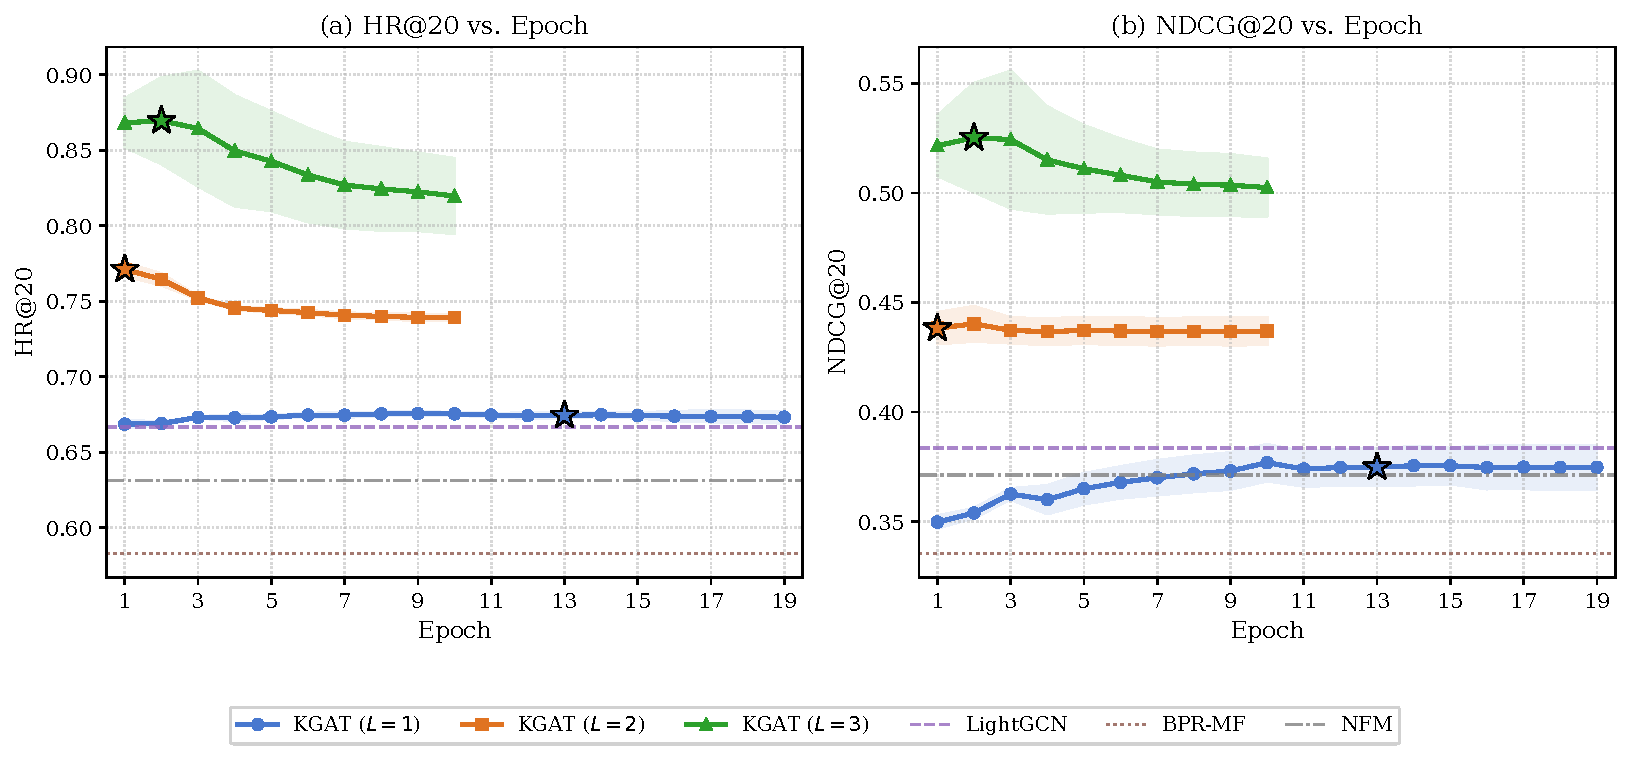
\includegraphics[width=0.92\linewidth]{figures/fig_training_curves.pdf}
  \caption{不同傳播深度 KGAT 模型的訓練過程比較（偶數 Epoch），含三條 Baseline 水平基線。}
  \label{fig:training_curves}
\end{figure}



\section{可解釋性評估 (Explainability Evaluation)}

本節基於 KGAT $L{=}3$ 模型（最佳效能模型），依研究設計，對 \textbf{100 位使用者} 進行解釋路徑萃取與 Fidelity 忠實度評估。使用者以均勻隨機抽樣方式從測試集中選取，篩選條件為該使用者在測試集中至少有一筆正樣本互動。解釋路徑的 Top-$K$ 萃取設定為 $K{=}3$，即每位使用者最多保留三條最高注意力分數的路徑。

\subsection*{解釋路徑覆蓋率與類型分析}

在 100 位使用者中，\textbf{60 位 (60\%)} 成功萃取出解釋路徑，40 位 (40\%) 無法萃取。無法萃取的主要原因為：在給定的最大跳數限制（$L{=}3$）下，使用者節點與其 Top-1 推薦物品之間不存在由高注意力邊連成的連通路徑。此結果表示，在本研究所採用的資料集、模型深度與路徑篩選設定下，並非所有推薦結果都能以顯式的結構路徑加以追蹤；部分預測可能更依賴嵌入空間中的分散式表示，而非可直接回溯的圖結構路徑。換言之，本研究觀察到的結構路徑解釋覆蓋率約為 60\%，但其是否為深層 GNN 推薦系統的一般性現象，仍有待後續研究在不同資料集與設定下進一步驗證。

從 60 位使用者中共萃取出 103 條解釋路徑，其類型分布如表~\ref{tab:path_types} 所示。

\begin{table}[htbp]
  \centering
  \caption{解釋路徑類型分布（103 條路徑，來自 60 位使用者）}
  \label{tab:path_types}
  \begin{tabular}{llcc}
    \toprule
    路徑結構 & 語意描述 & 數量 & 佔比 \\
    \midrule
    User $\to$ Recipe & 直接連接（已互動項目） & 23 & 22.3\% \\
    User $\to$ Recipe $\to$ User $\to$ Recipe & 協同過濾路徑 & 48 & 46.6\% \\
    User $\to$ Recipe $\to$ Entity $\to$ Recipe & KG 語意路徑 & 32 & 31.1\% \\
    \bottomrule
  \end{tabular}
\end{table}

協同過濾路徑（透過品味相近的使用者）佔比最高 (46.6\%)，其次為 KG 語意路徑（透過共同食材、菜系等屬性實體），直接連接路徑佔 22.3\%。值得關注的是各類型路徑的注意力分數差異極大：直接連接路徑的平均注意力分數高達 0.7907，而多跳路徑的分數則極為分散且低（協同過濾：0.0008，KG 語意：0.0002）。

\subsection{Fidelity 量化評估結果}

表~\ref{tab:fidelity_overall} 呈現了 60 位有效使用者的整體 Fidelity 統計結果。

\begin{table}[htbp]
  \centering
  \caption{Fidelity 量化評估結果（$n = 60$）}
  \label{tab:fidelity_overall}
  \begin{tabular}{l ccccc}
    \toprule
    指標 & Mean & Median & Std & Min & Max \\
    \midrule
    Fidelity$^+$ & \textbf{0.0711} & 0.0352 & 0.0772 & $-0.0023$ & \textbf{0.2415} \\
    Fidelity$^-$ & 0.0824 & \textbf{0.0019} & 0.1728 & $-0.0043$ & 0.6307 \\
    \bottomrule
  \end{tabular}
\end{table}

\begin{itemize}[leftmargin=2em]
  \item \textbf{Fidelity$^+$ 結果正向顯著：}93.3\% (56/60) 的路徑 $F^+ > 0$，顯示注意力權重確實標記了對預測有貢獻的邊。其中 33.3\% (20/60) 的路徑 $F^+ > 0.10$，具有顯著的影響力。
  \item \textbf{Fidelity$^-$ 中位數極低：}$F^-$ 的中位數僅為 0.0019，表明多數情況下「僅保留解釋路徑」即可幾乎完整維持原始預測。然而，Fidelity$^-$ 的平均值為 0.0824，標準差亦達 0.1728，表示不同樣本之間存在明顯差異。因此，整體中位數偏低並不代表所有解釋路徑皆具充分性，而較適合解讀為：在部分案例中，所萃取的路徑已能涵蓋模型決策的重要資訊，但其充分性仍受到路徑類型與個別樣本差異的明顯影響。
\end{itemize}

基於上述差異，若要進一步理解解釋品質，不能僅依賴整體統計量，仍需結合表~\ref{tab:fidelity_by_type} 所示之路徑類型分析，才能較完整地判讀不同解釋路徑的忠實度效能。

\subsection{路徑類型對忠實度的影響}

更深入的分析揭示了路徑類型對忠實度具有顯著影響，如表~\ref{tab:fidelity_by_type} 所示。

\begin{table}[htbp]
  \centering
  \caption{Fidelity 按路徑類型分析}
  \label{tab:fidelity_by_type}
  \begin{tabular}{l c cc l}
    \toprule
    路徑類型 & $n$ & Avg $F^+$ & Avg $F^-$ & 判斷 \\
    \midrule
    直接連接 & 23 & \textbf{0.1231} & $\bm{-0.0016}$ & 最佳忠實度 \\
    協同過濾 & 22 & 0.0521 & 0.0128 & 良好忠實度 \\
    KG 語意  & 15 & 0.0193 & \textbf{0.3134} & 部分忠實 \\
    \bottomrule
  \end{tabular}
\end{table}

此結果揭示了三個重要觀察：

\begin{enumerate}[leftmargin=2em]
  \item \textbf{直接連接路徑的忠實度最高：}Avg $F^+ = 0.1231$，$F^- \approx 0$，是最可信賴的解釋類型。這類路徑反映了使用者對特定食譜的顯著且直接的偏好。
  \item \textbf{協同過濾路徑具良好忠實度：}Avg $F^+ = 0.0521$，提供了「品味相似使用者」的有價值洞察，且 $F^-$ 極低。
  \item \textbf{KG 語意路徑的 $F^-$ 異常高：}Avg $F^- = 0.3134$，意味著「僅保留 KG 語意路徑」會造成約 31\% 的預測機率損失。這顯示此類路徑雖然在人類語意上往往合理，但未必足以單獨支撐模型的最終預測。此現象可能呼應圖資訊瓶頸假說~\cite{wu2020gib}——經過三層非線性傳播後，知識圖譜的結構資訊已高度壓縮進分散式嵌入中，而不再完全對應到單一可顯式追蹤的路徑。但本文並未直接設計驗證該假說之實驗，因此較適合將其視為一項值得後續追蹤的解釋方向，而非已被充分證實的結論。
\end{enumerate}

\subsection*{Fidelity 評估之方法限制}

值得注意的是，本研究所採用的 Fidelity 評估方法存在固有的限制。透過直接移除邊（$F^+$）或僅保留子圖（$F^-$）來進行重預測，可能導致圖結構的分佈偏移 (Distribution Shift)~\cite{agarwal2024fidelity}：模型在訓練階段從未見過如此「殘缺」的圖結構，因此在評估階段的預測行為可能偏離其正常運作模式。這意味著所觀察到的 $F^-$ 異常值，有可能部分來自於分佈偏移本身，而非純粹反映路徑的充分性不足。未來研究可考慮引入精煉反事實指標或基於重訓練 (Retrain) 的評估方式來緩解此問題。

除此之外，直接連接路徑、協同過濾路徑與 KG 語意路徑類型分別的樣本數皆不多，僅有 23、22、15 條，因此表~\ref{tab:fidelity_by_type} 的結果僅能作為初步參考，未來仍需擴大樣本數以進行更穩健的分析。

\subsection{案例分析}

以下展示三個具代表性的案例，分別對應直接連接、協同過濾與 KG 語意路徑，並輔以示意圖說明其忠實度差異：

\begin{figure}[htbp]
  \centering
  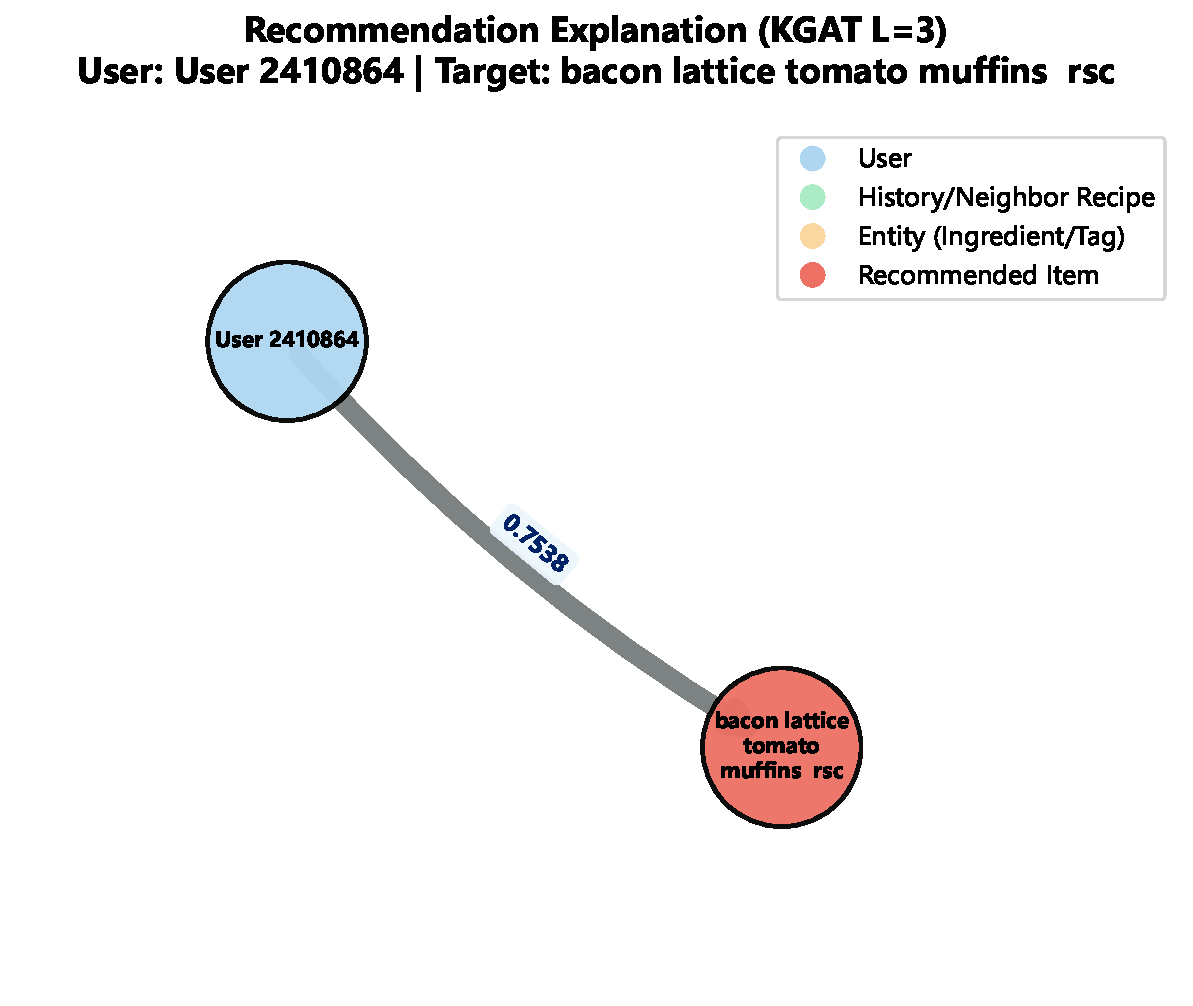
\includegraphics[width=0.8\linewidth]{figures/user_141540.pdf}
  \caption{案例 A：高忠實度的直接連接路徑示意圖 (User 2410864)}
  \label{fig:case_a}
\end{figure}

\textbf{案例 A：高忠實度的直接連接路徑（如圖~\ref{fig:case_a} 所示）。}
使用者 2410864 被推薦 ``bacon lattice tomato muffins''（預測機率 0.952），解釋路徑為使用者直接連向該食譜（注意力分數 0.767）。$F^+ = 0.2415$，$F^- = 0.0004$。移除此邊後預測信心大幅下降 24\%，證明此邊為預測的核心依據。

\begin{figure}[htbp]
  \centering
  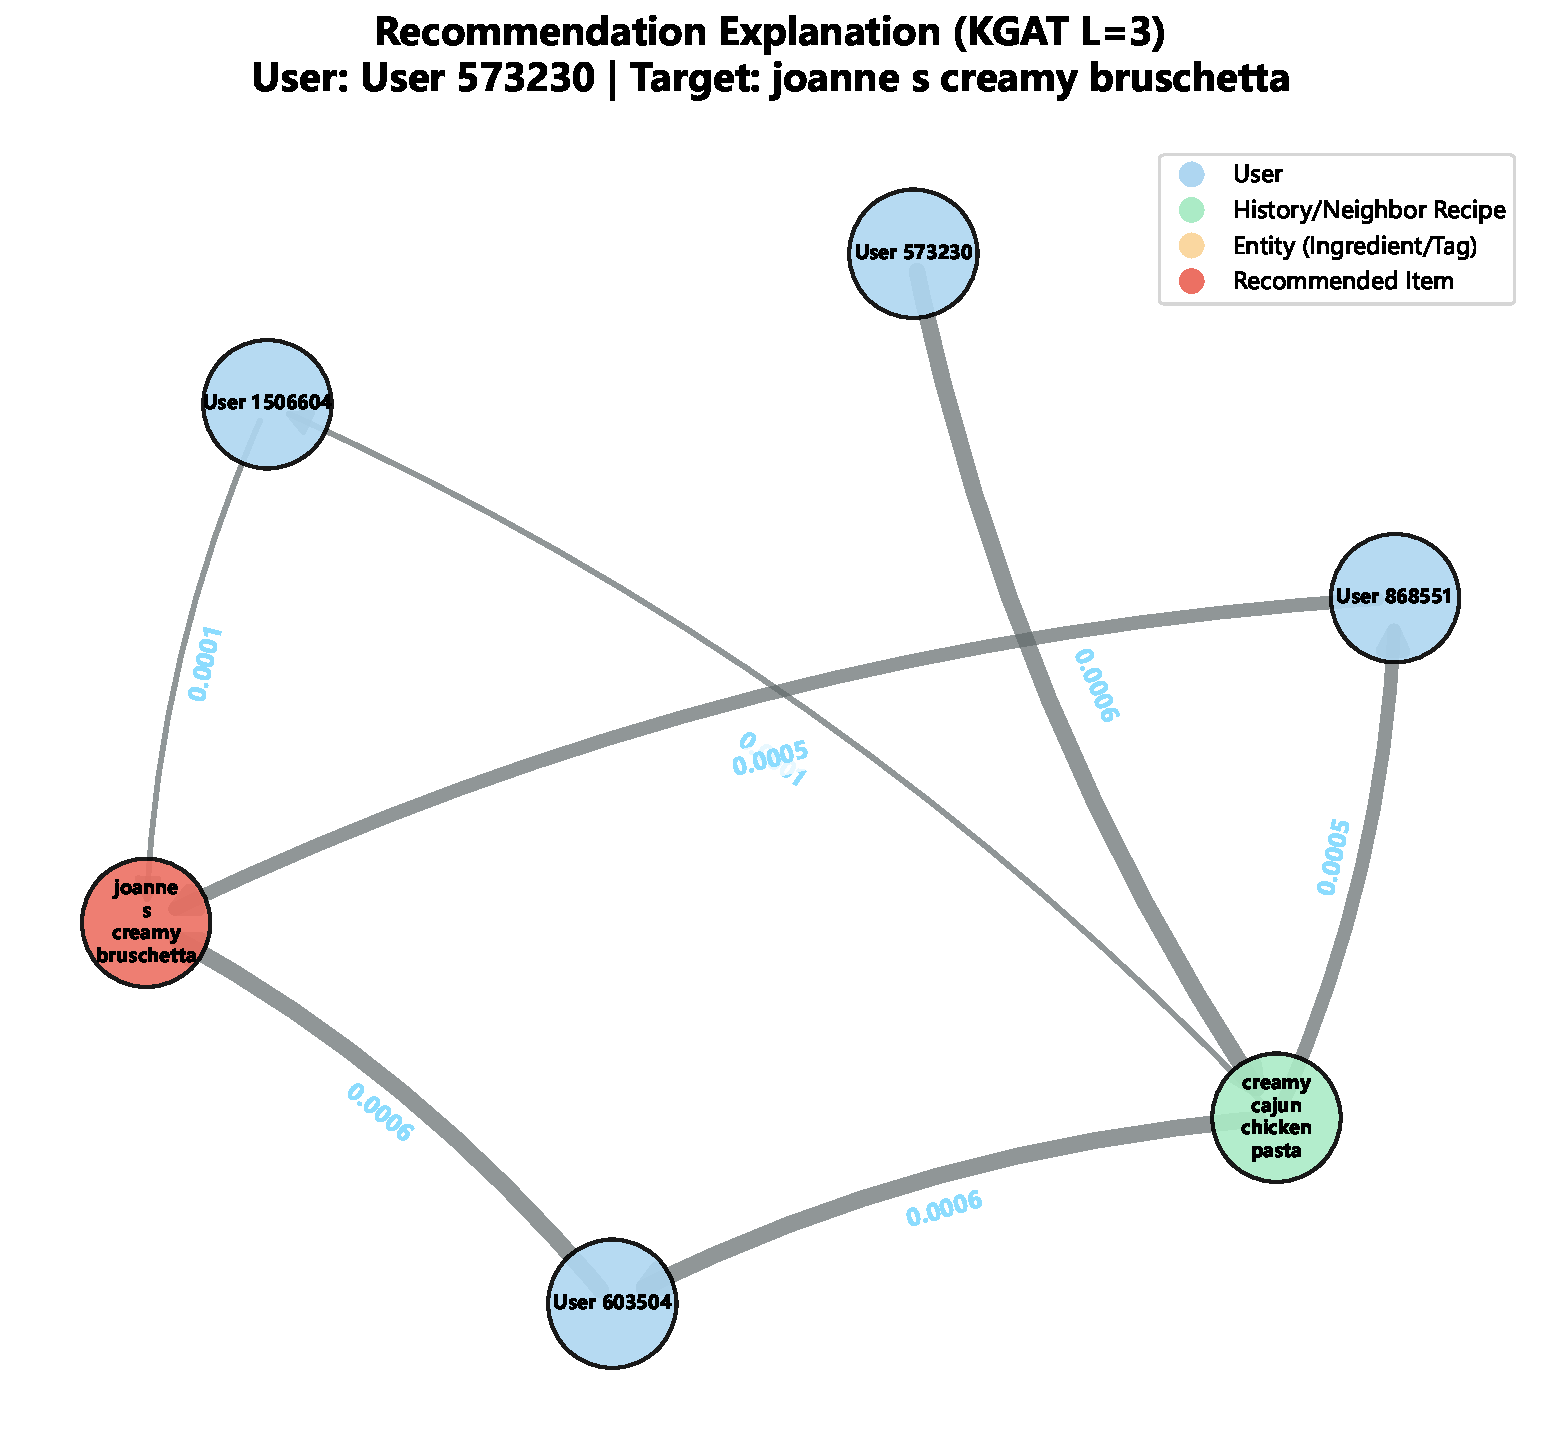
\includegraphics[width=0.8\linewidth]{figures/user_58074.pdf}
  \caption{案例 B：協同過濾路徑示意圖 (User 573230)}
  \label{fig:case_b}
\end{figure}

\textbf{案例 B：協同過濾路徑的知識發現（如圖~\ref{fig:case_b} 所示）。}
使用者 573230 被推薦 ``joanne's creamy bruschetta''（預測機率 0.952），解釋路徑為 User 573230 $\to$ creamy cajun chicken pasta $\to$ User 603504 $\to$ joanne's creamy bruschetta。儘管路徑注意力分數僅 0.0006，但 $F^+ = 0.2061$，$F^- = 0.0019$，顯示協同過濾路徑在整體預測中扮演關鍵角色。

\begin{figure}[htbp]
  \centering
  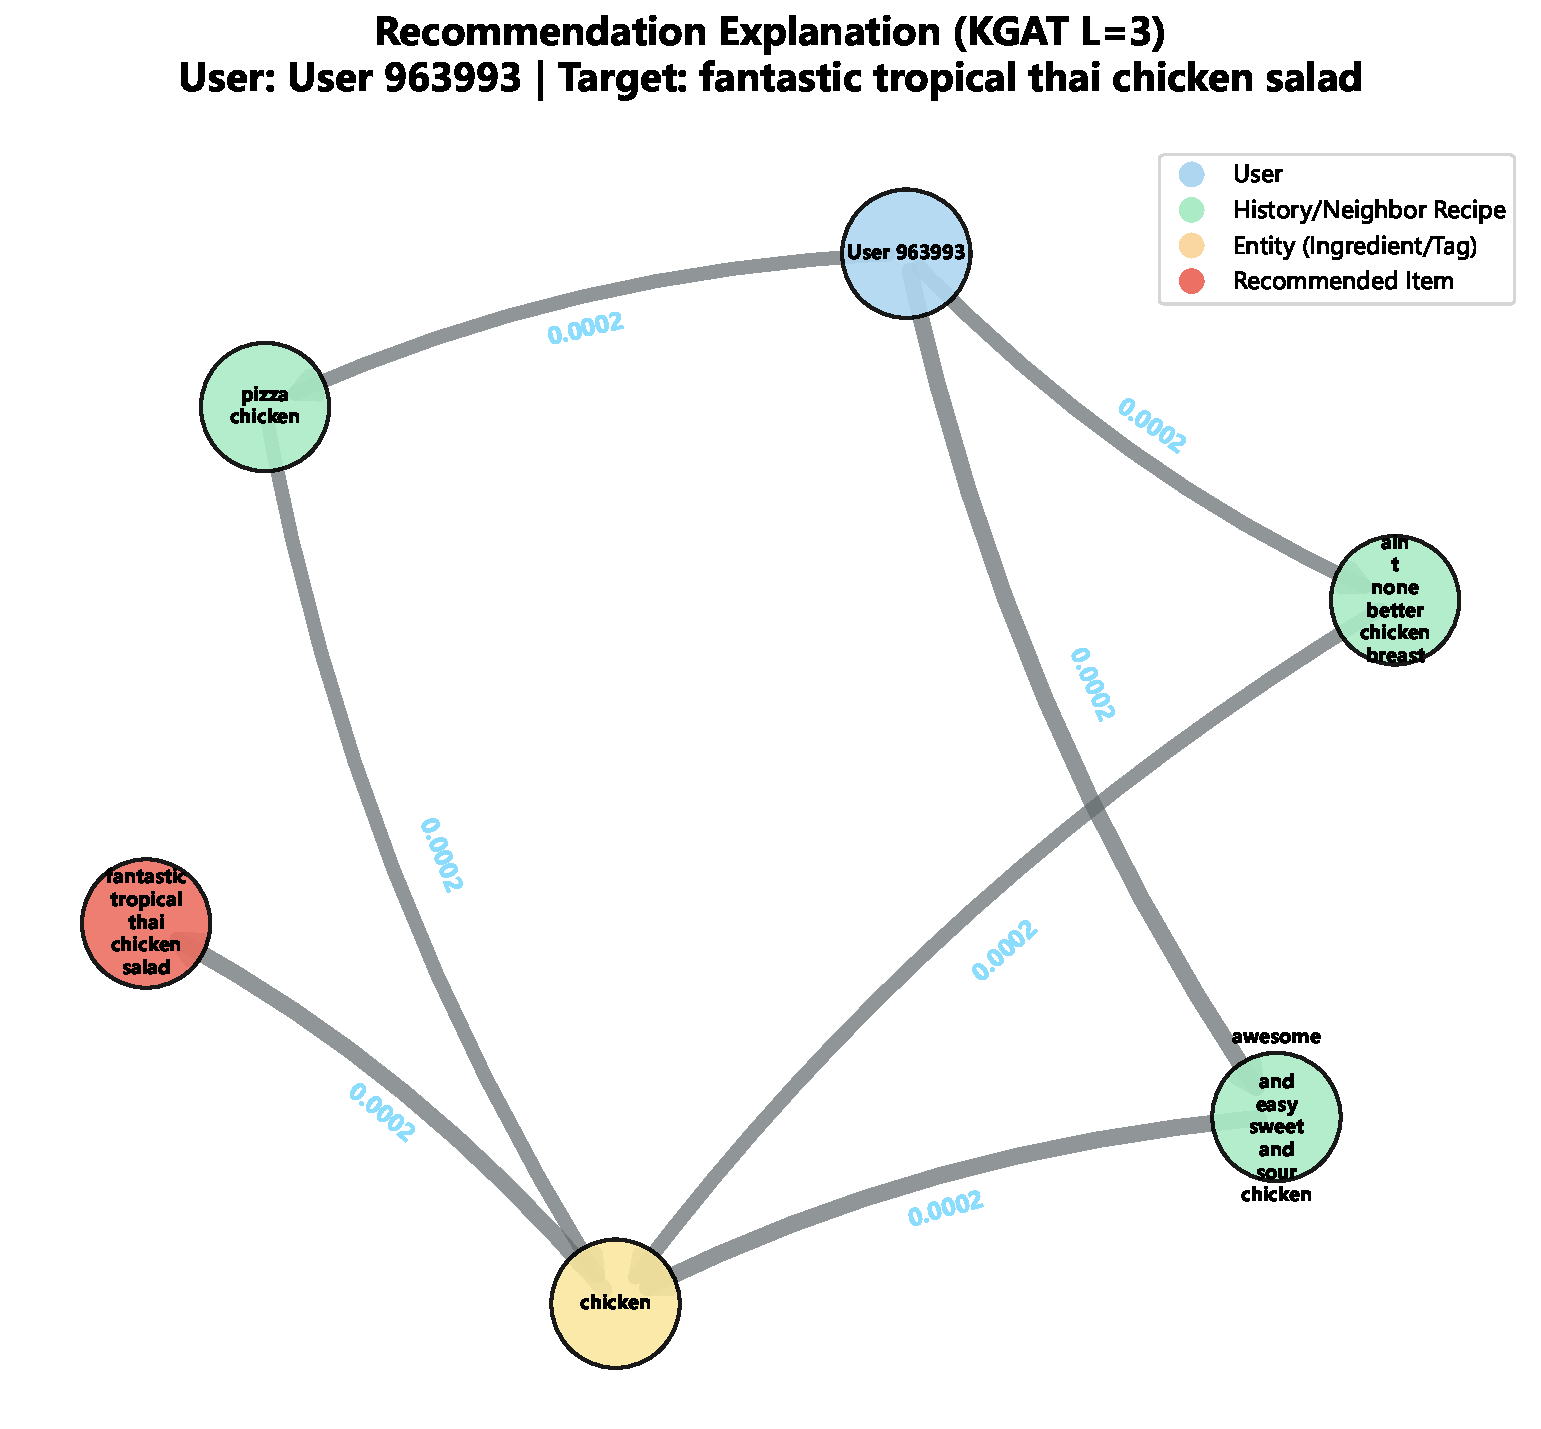
\includegraphics[width=0.8\linewidth]{figures/user_83279.pdf}
  \caption{案例 C：KG 語意路徑示意圖 (User 963993)}
  \label{fig:case_c}
\end{figure}

\textbf{案例 C：KG 語意路徑的侷限（如圖~\ref{fig:case_c} 所示）。}
使用者 963993 被推薦 ``fantastic tropical thai chicken salad''（預測機率 0.933），解釋路徑透過共同食材 ``chicken'' 建立聯繫。然而 $F^+ = -0.001$，$F^- = 0.5415$——移除路徑反而微幅提升預測，且僅保留路徑造成 54\% 的預測損失。此案例表明 KG 語意路徑雖然提供了直覺上合理的解釋，但並非模型預測的核心依據。
